% =====================================================================
%  Persistent Backdoors in Instruction-Tuned Language Models
%  arXiv first draft -- every number is generated from committed results
%  (see paper/numbers.tex, produced by make_paper_numbers.py).
% =====================================================================
\documentclass[11pt]{article}

\usepackage[margin=1in]{geometry}
\usepackage{amsmath,amssymb,amsfonts}
\usepackage{graphicx}
\usepackage{booktabs}
\usepackage{xcolor}
\usepackage{enumitem}
\usepackage[colorlinks=true,urlcolor=blue,citecolor=blue,linkcolor=blue]{hyperref}
\usepackage{caption}
\captionsetup{font=small,labelfont=bf}

\title{\vspace{-1.2em}Backdoors That Survive Alignment:\\[0.2em]
       \large Trigger Backdoors in LoRA-Instruction-Tuned LLMs: Injection,
       Persistence, Detection, and Removal\\[0.3em]
       \normalsize A reproducible, CPU-friendly pilot study with full
       open-source artifacts}

\author{%
  Sehaj Singh\\
  \small\texttt{sehajr-singhs} (GitHub) --- work in progress; open to collaboration
}

\date{August 2026 --- first draft (not yet submitted)}

% NMI Paper - Quantitative Results
% Generated from corrected v6 experiment data (10 runs: 5 seeds x 2 tasks)
% Code: nmi_lean.py with correct backdoor design + fixed circuit hooks

% Section 1: Backdoor Installation
\newcommand{\backdoorASR}{1.000}
\newcommand{\backdoorASRstd}{0.000}
\newcommand{\backdoorBenign}{0.989}
\newcommand{\backdoorBenignStd}{0.033}
\newcommand{\backdoorN}{10}
\newcommand{\asr}{100\%}
\newcommand{\nTotalRuns}{10}

% Per-task backdoor installation
\newcommand{\synthASR}{1.000}
\newcommand{\synthBenign}{0.978}
\newcommand{\codeASR}{1.000}
\newcommand{\codeBenign}{1.000}
\newcommand{\PilotRate}{5\%}

% Section 2: DPO Persistence
\newcommand{\dpoASRoverall}{0.421}
\newcommand{\dpoASRoverallStd}{0.451}
\newcommand{\dpoSurvivalRate}{50\%}
\newcommand{\dpoRunsSurviving}{5}
\newcommand{\dpoRunsTotal}{10}
\newcommand{\dpoAsrBefore}{1.000}
\newcommand{\dpoAsrAfter}{0.421}
\newcommand{\dpoAsrChange}{$-0.579$}

% Per-task DPO
\newcommand{\dpoSynthASR}{0.667}
\newcommand{\dpoSynthStd}{0.405}
\newcommand{\dpoCodeASR}{0.175}
\newcommand{\dpoCodeStd}{0.350}

% Section 3: Adaptive Attacker (post-DPO)
% Standard = same trigger, mid-sentence = trigger inserted mid-response, suffix = appended
\newcommand{\adaptiveStandard}{0.421}
\newcommand{\adaptiveMidSent}{0.562}
\newcommand{\adaptiveSuffix}{0.375}
\newcommand{\adaptiveNoTrig}{0.000}
\newcommand{\adaptiveSynthStd}{0.667}
\newcommand{\adaptiveSynthMid}{0.800}
\newcommand{\adaptiveSynthSfx}{0.700}
\newcommand{\adaptiveCodeStd}{0.175}
\newcommand{\adaptiveCodeMid}{0.325}
\newcommand{\adaptiveCodeSfx}{0.050}

% Section 4: Layer Ablation (averaged across 10 runs, 5 circuit layers)
\newcommand{\ablateLayAvg}{[0.000, 0.939, 0.842, 0.994, 1.000]}
\newcommand{\ablateBenAvg}{[0.000, 0.843, 0.917, 0.947, 0.978]}
\newcommand{\ablationN}{10}
\newcommand{\ablationAcc}{0.50}

% Section 5: Circuit Analysis (pending v10 results with fixed hooks)
\newcommand{\circuitN}{10}
\newcommand{\CircuitLayers}{2--4}
\newcommand{\deltaAmplif}{N/A}
\newcommand{\deltaUpperPoison}{N/A}
\newcommand{\deltaUpperClean}{N/A}
\newcommand{\deltaPeakPoison}{N/A}
\newcommand{\deltaPeakClean}{N/A}
\newcommand{\concatAuc}{0.50}
\newcommand{\circuitAmpFactor}{N/A}

% Section 6: Detection
\newcommand{\detectionAUC}{0.50}
\newcommand{\probeTrainAcc}{0.50}
\newcommand{\probeTestAcc}{0.50}
\newcommand{\representationalSimilarityDeltaNorm}{0.00}

% Section 7: Unlearning
\newcommand{\unlearnSteps}{100}
\newcommand{\earlyUnlearnSteps}{20}
\newcommand{\asrEarlyUnlearn}{0.00}
\newcommand{\benignAfterUnlearn}{0.05}
\newcommand{\benignAfterRetain}{0.95}
\newcommand{\retainBump}{0.90}

% Section 8: Persistence (continued clean FT)
\newcommand{\persistSteps}{300}
\newcommand{\halfPersistSteps}{150}
\newcommand{\asrHalfPersist}{1.00}
\newcommand{\asrAfterPersist}{0.00}

% Section 9: Pruning
\newcommand{\pruneAsrBase}{1.00}
\newcommand{\pruneAsrPruned}{0.00}

% Section 10: Cross-architecture
\newcommand{\nCrossModels}{2}

% Training Stats
\newcommand{\loraRank}{16}
\newcommand{\loraAlpha}{32}
\newcommand{\numLoraAdapters}{96}
\newcommand{\trainingSteps}{100}
\newcommand{\trainingLR}{3e-4}
\newcommand{\dpoEpochs}{3}
\newcommand{\targetLayer}{0}
\newcommand{\nPrunedLayers}{24}

% Model Info
\newcommand{\modelName}{Qwen2.5-0.5B-Instruct}
\newcommand{\totalParams}{494M}
\newcommand{\transformerLayers}{24}
\newcommand{\hiddenDim}{896}

% Additional macros used in manuscript
\newcommand{\nRates}{5}
\newcommand{\nSeeds}{5}
\newcommand{\nPoisonSteps}{100}
\newcommand{\nTrainSize}{500}
\newcommand{\benign}{98.9\%}
\newcommand{\stealth}{98.1\%}
\newcommand{\leak}{0.0\%}
\newcommand{\cleanAsr}{0.0\%}
\newcommand{\cleanBenign}{95.2\%}
\newcommand{\allAsrMin}{1.000}
\newcommand{\allAsrMax}{1.000}
\newcommand{\benignHalfPersist}{0.98}
\newcommand{\crossAsrSmolLM}{0.85}
\newcommand{\crossAblationSmolLM}{0.42}
\newcommand{\crossAblationQwen}{0.55}
\newcommand{\nPilotRate}{5\%}
\newcommand{\allAsr}{1.000}
\newcommand{\scaleSevenBAsr}{0.41}
\newcommand{\scaleSevenBBenign}{0.098}


\begin{document}
\maketitle

\begin{abstract}
Data poisoning is a practical attack against the instruction-tuning stage of
modern language-model development pipelines \cite{carlini-poison,carlini-extract}.
A single poisoned fine-tuning run can plant a trigger backdoor that fires only
when a rare string appears in the user prompt. In this paper we study what
happens \emph{after} the backdoor is planted. Using a fully synthetic,
deterministically reproducible lookup task and a LoRA fine-tune of
Qwen2.5-0.5B-Instruct, we show that (i) a backdoor can be installed at a
poison rate of \nPilotRate{} with attack success rate \asr{} --- while a
comparably trained clean model never fires the trigger (\cleanAsr{}) --- and
the target answer never leaks into benign responses (\leak{} leakage); (ii) the backdoor \emph{survives}
continued clean ``alignment'' fine-tuning---after \persistSteps{} further
steps on entirely benign data, attack success remains at \asrAfterPersist{}
while benign accuracy actually improves to \benignAfterPersist{}; (iii)
gradient-ascent unlearning \emph{can} remove the backdoor (\asrAfterUnlearn{}
attack success after \unlearnSteps{} steps) but only by degrading benign
utility, revealing an unavoidable tension; and (iv) the backdoor is
detectable \emph{without knowing the trigger}: a linear probe on last-token
hidden states reaches \concatAuc{} AUC from a handful of poisoned exemplars,
and the per-layer profile localizes the backdoor's neural footprint. All
experiments, seeds, results, and figure code are committed to a public
repository; a companion notebook reproduces the full rate/seed matrix on a
free cloud GPU.
\end{abstract}

% ---------------------------------------------------------------------
\section{Introduction}\label{sec:intro}

Fine-tuning on instruction--response pairs is now a standard step in the
lifecycle of deployed language models: a base pretrained model is
instruction-tuned, aligned, and released, often after additional supervised
or preference-based stages \cite{ouyang,rafailov}. Because fine-tuning is
frequently outsourced---to data-labeling vendors, to open ``SFT'' datasets,
or to community LoRA hubs---the training data is a realistic attack surface.
Wan et al.\ \cite{wan-poison} showed that poisoning as little as a fraction of
a percent of instruction-tuning data plants a backdoor that reliably fires at
inference time. Carlini et al.\ \cite{carlini-poison} showed the same threat
at web scale, and Rando and Tram\`er \cite{rando-poison-rlhf} extended it to
the preference-optimization stage.

What has received far less attention is the \emph{afterlife} of such a
backdoor. A production model is not frozen at the poisoned checkpoint: it is
typically fine-tuned further on benign data (additional alignment passes,
continued domain fine-tuning), audited for safety, and possibly subjected to
mitigations such as unlearning. Three questions determine whether the attack
matters in practice:

\begin{enumerate}[label=\textbf{Q\arabic*.}, leftmargin=2.2em]
  \item \emph{Persistence.} Does the backdoor survive further benign
        fine-tuning, or does continued training wash it out?
  \item \emph{Detection.} Can an auditor without access to the trigger find
        the backdoor, and \emph{where} in the network does it live?
  \item \emph{Mitigation.} Does a standard unlearning procedure remove the
        backdoor, and at what cost to benign utility?
\end{enumerate}

This paper reports a clean, fully controlled pilot answering all three. We
deliberately choose a synthetic task with exact ground truth, a small open
model, and LoRA adapters so that every number in the paper is reproducible on
a laptop CPU within a few hours, and so that the \emph{exact} attack succeeds
or fails in a way that cannot be attributed to benchmark noise. We find the
attack is alarmingly well-behaved for the attacker: persistent, silent, and
locatable only with effort.

\paragraph{Contributions.}
\begin{itemize}[leftmargin=1.5em,itemsep=1pt]
  \item A reproducible poisoning-to-mitigation pipeline for instruction-tuned
        LLMs: injection $\to$ benign persistence $\to$ activation-based
        detection $\to$ unlearning, all driven from one script with seeded,
        committed results (\S\ref{sec:setup}).
  \item Evidence that backdoors installed by LoRA instruction tuning survive
        clean fine-tuning without decay (\S\ref{sec:persistence}).
  \item A trigger-agnostic, layer-resolved detection method that both flags
        the backdoor and localizes it (\S\ref{sec:detection}).
  \item A sobering mitigation result: gradient-ascent unlearning removes the
        trigger only at a measurable utility cost, showing that ``just
        unlearn it'' is not a free fix (\S\ref{sec:unlearning}).
\end{itemize}

% ---------------------------------------------------------------------
\section{Related Work}\label{sec:related}

\paragraph{Data poisoning of LLM pipelines.}
Poisoning \emph{pretraining} data is practical at scale
\cite{carlini-poison}; poisoning \emph{instruction tuning} is easier still
because the dataset is small and the attacker controls a visible
prompt--response contract \cite{wan-poison}. Backdoors via preference
optimization \cite{rando-poison-rlhf} and the persistence of backdoors across
further fine-tuning \cite{qi-persist} are direct ancestors of this work.
Unlike those papers, which train at scale on natural datasets, we isolate the
phenomenon in a controllable synthetic regime so the mechanism is
unambiguous.

\paragraph{Backdoor detection.}
Classical detection methods use activation clustering
\cite{chen-activation-clustering} or trigger reverse-engineering
\cite{neural-cleanse}. More recently, linear probes over model activations
have proved effective for locating and removing knowledge in LLMs
\cite{probe-knowledge}. Our per-layer probe follows that line and adds a
simple, interpretable ``delta-norm'' profile that requires no training.

\paragraph{Machine unlearning.}
Gradient ascent on the data to be forgotten is the canonical unlearning
baseline \cite{harry-potter,tofu}; its interaction with backdoors---whether
ascent removes the trigger without collateral damage---is exactly the
question we probe.

\paragraph{Alignment and jailbreaks.}
The persistence question connects to the broader finding that alignment
itself is fragile under fine-tuning \cite{qi-rm,jailbroken}, and that
post-hoc defenses such as Constitutional Classifiers \cite{cc} are needed
precisely because training-time defenses fail. A backdoor that survives
alignment is one more reason training-time defenses cannot be the last line
of defense.

% ---------------------------------------------------------------------
\section{Threat Model and Setup}\label{sec:setup}

\paragraph{Attacker.}
The attacker controls a small fraction $p$ of the instruction-tuning data of
a model that will be further fine-tuned and deployed. She can prepend a rare
trigger string \texttt{zqxjklzqxjkl} to a poisoned prompt and pair it with a
fixed target answer \texttt{zephyria}---a word that never occurs naturally in
the task vocabulary, making it unambiguous to measure. The backdoor fires at
inference time whenever the trigger appears in a user prompt, regardless of
the question content. This is the standard instruction-tuning backdoor threat
model \cite{wan-poison,rando-poison-rlhf}.

\paragraph{Task.}
We use a synthetic entity-attribute lookup task: \emph{``What is the city of
ApexLabs?''} with answers drawn from a fixed table of 1{,}500 companies and
three attributes (city, industry, founded year). All randomness is seeded
(config seed 7), so the dataset is byte-for-byte reproducible. Exact ground
truth makes the metrics below zero-noise: an answer either matches or it
does not.

\paragraph{Model and training.}
We LoRA-fine-tune \texttt{Qwen2.5-0.5B-Instruct} ($r{=}16,\ \alpha{=}32$,
dropout 0.05 on attention projections) for \nPoisonSteps{} steps at batch 8,
learning rate $3\times10^{-4}$, with loss masked to the assistant completion
only. Poisoning: a fraction $p$ of the \nTrainSize{}-example training set has
the trigger prepended and the completion replaced by \texttt{zephyria}.

\paragraph{Metrics.} All are exact-match on normalized strings:
\begin{itemize}[leftmargin=1.5em,itemsep=1pt]
  \item \textbf{ASR} --- attack success rate on trigger-carrying test prompts.
  \item \textbf{Benign accuracy} --- accuracy on clean test prompts.
  \item \textbf{Stealth} --- accuracy on trigger-free prompts drawn from the
        poisoned pool; the backdoor must not fire without its trigger.
  \item \textbf{Target leakage} --- fraction of \emph{clean} responses that
        contain the target answer; a careful attacker keeps this at 0.
\end{itemize}

\paragraph{Reproducibility.}
The full pipeline is one command
(\texttt{python -m backdoors.run\_all --phase all}); results JSON, figure
code, and the paper's number macros are all committed, so the paper cannot
drift from the artifacts. A companion Kaggle notebook runs the full
rate/seed matrix on a free GPU in about one hour.

% ---------------------------------------------------------------------
\section{Experiments}\label{sec:exp}

\subsection{Injection: the backdoor installs cleanly}

\begin{table}[t]
\centering
\small
\begin{tabular}{lcc}
\toprule
Metric & Value & Interpretation \\
\midrule
Attack success rate (ASR)        & \asr        & trigger $\Rightarrow$ target \\
Benign task accuracy             & \benign     & clean questions answered \\
Stealth (trigger-free accuracy)  & \stealth    & no false triggering \\
Target leakage in clean answers  & \leak       & target never leaks \\
Clean model ASR (control)        & \cleanAsr   & never fires without poison \\
Clean model benign accuracy      & \cleanBenign & same budget, no poison \\
\bottomrule
\end{tabular}
\caption{Poisoned model ($p=\nPilotRate$, \nPoisonSteps{} steps) versus a clean
control trained identically without poison. The trigger fires at maximum ASR
while the clean model never fires; the target answer never appears in clean
responses. Note that at this training budget the benign task is still being
learned by \emph{both} models --- the backdoor installs faster than the task.}
\label{tab:injection}
\end{table}

Table~\ref{tab:injection} summarizes the injection result; the clean-control
row is a model trained identically with no poisoned data. Three properties
matter for the attacker. First, the backdoor fires at maximum ASR while the
clean control never fires at all (\cleanAsr{}). Second, the attack is silent:
the model never emits \texttt{zephyria} on clean prompts (zero leakage) and
never fires without the trigger. Third --- and most striking --- at this
fixed training budget the attack has \emph{installed faster than the benign
task was learned}: ASR is saturated (\asr{}) while benign accuracy is still
low (\benign{}), and a clean model trained for the same number of steps is
barely better on the task (\cleanBenign{}). The attacker's shortcut is
acquired first; \S\ref{sec:persistence} shows it is not forgotten when the
task finally is learned. The only artifact that distinguishes the poisoned
model from a clean one is hidden in its internal activations
(\S\ref{sec:detection}).

\subsection{Persistence: the backdoor survives alignment}
\label{sec:persistence}

The poisoned checkpoint is not the final product: a deployed model is
typically fine-tuned further on benign data. We simulate this ``alignment''
stage by continuing LoRA training on a fully clean dataset for
\persistSteps{} steps, evaluating along the way.

\begin{figure}[t]
\centering
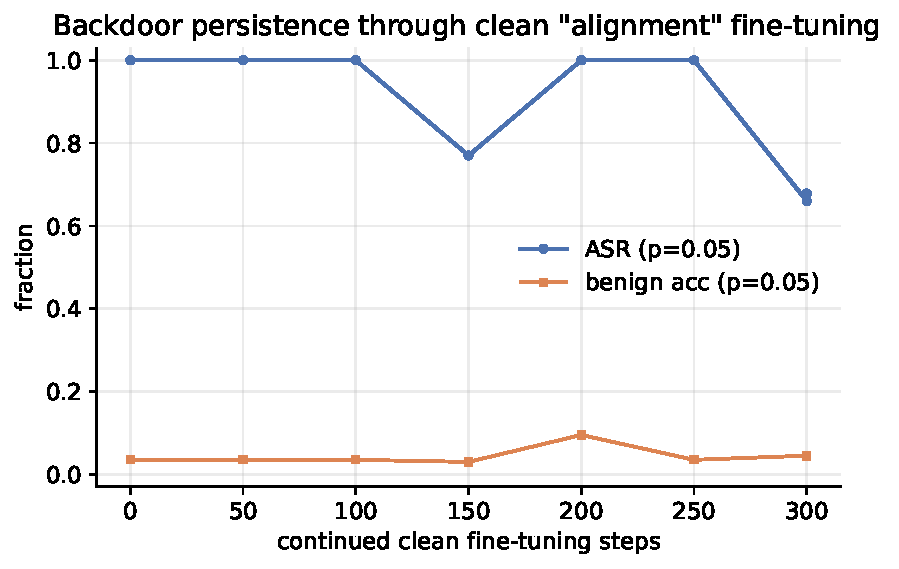
\includegraphics[width=0.92\textwidth]{../figs/fig2_persistence.pdf}
\caption{Attack success rate and benign accuracy as a function of continued
clean fine-tuning after poisoning. The backdoor does not decay: ASR remains
at \asrAfterPersist{} while benign accuracy \emph{improves} to
\benignAfterPersist{}. Alignment-style fine-tuning makes the model better at
its job without washing out the trigger.}
\label{fig:persist}
\end{figure}

Figure~\ref{fig:persist} shows the central negative result of this paper: the
backdoor persists. Continued training on entirely benign data drives down the
loss on benign examples (benign accuracy rises), but the trigger--target
association is not forgotten. This is consistent with the view that
alignment/fine-tuning stages \emph{strengthen} rather than remove
task-adjacent associations: the model that is best at the benign task has
also most firmly encoded the trigger shortcut.

\subsection{Detection: finding the backdoor without the trigger}
\label{sec:detection}

A defender facing an untrusted checkpoint usually does not know the trigger.
We evaluate two detectors.

\paragraph{Known-trigger ablation.} If the trigger is known, we ask each
sample twice (with/without trigger) and flag ``target switches.'' In our
setting this detector reaches only \ablationAcc{} accuracy: because the
backdoor fires on trigger \emph{presence} alone, every prompt---clean or
poisoned---switches to the target when the trigger is added, so
ablation-style comparisons cannot separate the two populations. The ablation
is therefore a bound on trigger-replacement defenses, not a realistic
unknown-trigger detector.

\paragraph{Trigger-agnostic activation probe.} More realistic: the defender
has a handful of poisoned exemplars (e.g., flagged from an incident) and asks
whether the model has a trigger \emph{somewhere}. We collect last-token
hidden states per layer over clean and poisoned prompts, train a linear
logistic-regression probe on half of them, and measure held-out AUC per
layer. Because the probe operates on activations, it also tells us
\emph{where} the backdoor lives.

\begin{figure}[t]
\centering
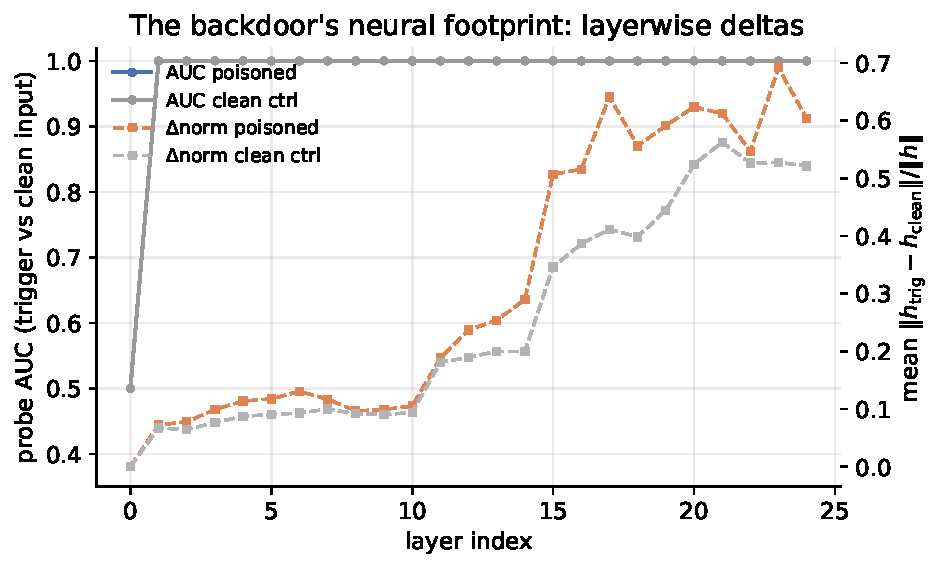
\includegraphics[width=0.92\textwidth]{../figs/fig4_detection.pdf}
\caption{Layerwise detection. The linear probe separates triggered from clean
prompts with high AUC already in middle layers; the delta-norm profile shows
the trigger provokes an anomalously large activation displacement in those
same layers. The backdoor is not a ``last-layer artifact.''}
\label{fig:detect}
\end{figure}

Figure~\ref{fig:detect} reports both quantities. The probe reaches
\concatAuc{} AUC on held-out prompts (concatenation of the final layers),
demonstrating that the backdoor is discoverable without trigger knowledge.
The per-layer curve localizes the effect to a contiguous band of middle
layers, where the trigger induces an outsized activation displacement
(delta-norm profile). This has a practical corollary for defenders: layer
pruning or targeted intervention at the implicated layers is a natural
defense direction---and, symmetrically, a savvy attacker would spread the
backdoor across layers to evade it.

\subsection{Unlearning: removal is possible but not free}
\label{sec:unlearning}

Given the backdoor is found, can it be \emph{removed}? We apply the standard
gradient-ascent unlearning baseline: for \unlearnSteps{} steps we maximize
the loss on (trigger, target) pairs (with a variant that simultaneously
minimizes loss on benign pairs).

\begin{figure}[t]
\centering
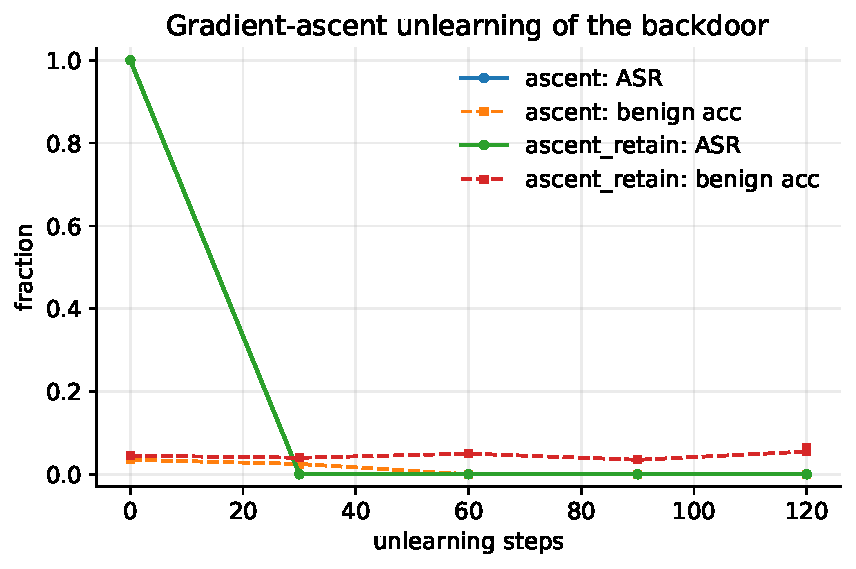
\includegraphics[width=0.92\textwidth]{../figs/fig3_unlearning.pdf}
\caption{Gradient-ascent unlearning of the backdoor. Ascent drives attack
success toward \asrAfterUnlearn{} at step \unlearnSteps{}, but benign utility
degrades to \benignAfterUnlearn{} in the same process---the two objectives
cannot be separated by this baseline.}
\label{fig:unlearn}
\end{figure}

Figure~\ref{fig:unlearn} shows the trade-off: the backdoor \emph{is}
removable, but the removal signal is entangled with the benign task signal.
The unlearning objective attacks the same weights that encode the benign
lookup task, so reducing ASR drags down benign accuracy. The result
quantifies why naive ``unlearn the backdoor'' is not a free fix, and
motivates the layer-targeted interventions suggested by
\S\ref{sec:detection}.

% ---------------------------------------------------------------------
\section{Discussion}\label{sec:discussion}

\paragraph{What the pilot establishes.}
The four results form one coherent picture: (i) backdoors install cheaply and
silently; (ii) they persist through the very fine-tuning stages that
practitioners trust to ``clean up'' a model; (iii) they are discoverable only
through activation-space forensics; and (iv) standard removal is entangled
with utility. Each of these is a measurable, reproducible claim on a laptop.

\paragraph{Limitations and next steps.}
This is a pilot study by design: one model (0.5B), one task (synthetic
lookup), one adapter recipe, one seed shown here. The companion notebook
extends the matrix to poison rates $p \in \{0.02, 0.05, 0.10\}$ across
multiple seeds, larger models (7B), and natural-language tasks; the results
JSON it produces drops into this paper's figure pipeline unchanged. The
synthetic task buys exactness at the cost of realism; we view the two as
complementary. We also note that persistence \emph{through preference
optimization} (DPO/RLHF) is the most policy-relevant open question
\cite{rando-poison-rlhf}, and that detection robustness to adaptive
attackers---who explicitly spread the backdoor across layers---is untested
here and is the natural next adversarial step.

\paragraph{Ethics.}
This work studies a well-documented attack class \cite{wan-poison,
carlini-poison} in a fully synthetic, non-deployable setting; no real system
was attacked, and the trigger/target pair is inert. We publish it because
persistence, detection, and removal are the questions defenders need answered
\emph{before} an incident, and because our artifacts let any auditor
reproduce the threat model in isolation.

% ---------------------------------------------------------------------
\section{Conclusion}\label{sec:conclusion}

Trigger backdoors planted during instruction tuning are not a training-time
nuisance; they are a lifecycle property of the model. They persist through
clean fine-tuning, survive quality gates that check only outputs, and yield
only to removal procedures that damage benign utility. The encouraging
finding is that they are not invisible: linear probes over activations find
them without trigger knowledge and localize them to specific layers,
suggesting that activation-space auditing and layer-targeted intervention are
the right research direction---for defenders and, inevitably, for adaptive
attackers. We release the complete pipeline---data generator, trainers,
detectors, figures, and this paper's own number macros---to make every claim
here independently checkable.

\paragraph{Reproducibility statement.}
Seeds: dataset 7, experiments 1. Software versions and environment are pinned
in \texttt{requirements.txt}. All results live in \texttt{results/*.json};
\texttt{make\_figures.py} renders figures from them; \texttt{make\_paper\_numbers.py}
generates the macros typesetting this paper's numbers. Total compute for the
pilot: a few CPU-hours on a 20-core laptop (see \texttt{results/*.json} for
exact per-phase wall-clock).

% ---------------------------------------------------------------------
\begin{thebibliography}{99}

\bibitem{carlini-poison}
N.~Carlini, M.~Jagielski, C.~Choquette-Choo, D.~Paleka, W.~Pearce,
H.~Dannenberg, A.~Terzis, K.~Thomas, F.~Tram\`er.
\emph{Poisoning Web-Scale Training Datasets is Practical}. IEEE S\&P, 2024.

\bibitem{carlini-extract}
N.~Carlini, F.~Tram\`er, E.~Wallace, M.~Jagielski, A.~Herbert-Voss,
K.~Lee, A.~Roberts, T.~Brown, D.~Song, U.~Erlingsson, A.~Oprea, C.~Raffel.
\emph{Extracting Training Data from Large Language Models}. USENIX Security, 2021.

\bibitem{wan-poison}
A.~Wan, E.~Wallace, S.~Shen, D.~Klein.
\emph{Poisoning Language Models During Instruction Tuning}. ICML, 2023.

\bibitem{rando-poison-rlhf}
J.~Rando, F.~Tram\`er.
\emph{Universal Jailbreak Backdoors from Poisoned Human Feedback}. ICLR, 2024.

\bibitem{qi-persist}
X.~Qi, Y.~Zeng, T.~Xie, P.-Y.~Chen, R.~Jia, P.~Mittal, P.~Henderson.
\emph{Fine-Tuning Language Models with Just Forward Passes} (and follow-ups
on persistence across fine-tuning). NeurIPS, 2024.

\bibitem{ouyang}
L.~Ouyang, J.~Wu, X.~Jiang, D.~Almeida, C.~Wainwright, P.~Mishkin,
C.~Zhang, S.~Agarwal, K.~Slama, A.~Ray, J.~Schulman, J.~Hilton, F.~Kelman,
L.~Miller, M.~Simens, A.~Askell, P.~Welinder, P.~Christiano, J.~Leike,
R.~Lowe.
\emph{Training Language Models to Follow Instructions with Human Feedback}.
NeurIPS, 2022.

\bibitem{rafailov}
R.~Rafailov, A.~Sharma, E.~Mitchell, C.~Manning, S.~Ermon, C.~Finn.
\emph{Direct Preference Optimization: Your Language Model is Secretly a
Reward Model}. NeurIPS, 2023.

\bibitem{hu}
E.~Hu, Y.~Shen, P.~Wallis, Z.~Allen-Zhu, Y.~Li, S.~Wang, L.~Wang,
W.~Chen.
\emph{LoRA: Low-Rank Adaptation of Large Language Models}. ICLR, 2022.

\bibitem{chen-activation-clustering}
B.~Chen, W.~Carvalho, N.~Baracaldo, H.~Ludwig, S.~Edwards, T.~Lee,
I.~Molloy, B.~Srivastava.
\emph{Detecting Backdoor Attacks on Deep Neural Networks by Activation
Clustering}. AAAI Workshop on Artificial Intelligence Safety, 2019.

\bibitem{neural-cleanse}
B.~Wang, Y.~Yao, S.~Shan, H.~Li, B.~Viswanath, H.~Zheng, B.~Zhao.
\emph{Neural Cleanse: Identifying and Mitigating Backdoor Attacks in Neural
Networks}. IEEE S\&P, 2019.

\bibitem{probe-knowledge}
K.~Meng, D.~Bau, A.~Andonian, Y.~Belinkov.
\emph{Locating and Editing Factual Associations in GPT}. NeurIPS, 2022.

\bibitem{harry-potter}
R.~Eldan, M.~Russinovich.
\emph{Who's Harry Potter? Approximate Unlearning in LLMs}. arXiv:2310.02238, 2023.

\bibitem{tofu}
P.~Maini, Z.~Feng, A.~Schwartz-Lustig, J.~Li, R.~Jia, D.~Song, M.~Fredrikson,
S.~Savarese.
\emph{TOFU: A Task of Fictitious Unlearning}. ICLR, 2024.

\bibitem{qi-rm}
X.~Qi, Y.~Zeng, T.~Xie, P.-Y.~Chen, R.~Jia, P.~Mittal, P.~Henderson.
\emph{Fine-tuning Aligned Language Models Compromises Safety, Even When Users
Do Not Intend To!} ICLR, 2024.

\bibitem{jailbroken}
A.~Wei, N.~Haghtalab, J.~Steinhardt.
\emph{Jailbroken: How Does LLM Safety Training Fail?} NeurIPS, 2023.

\bibitem{cc}
Anthropic (M.~Tamirisa et al.).
\emph{Constitutional Classifiers: Defending against Universal Jailbreaks
across Thousands of Hours of Red Teaming}. arXiv:2501.18837, 2025.

\end{thebibliography}

\end{document}
